\chapter{天球}
\section{地心说}
古希腊人最早根据观测直觉,认为天体围绕地球转,提出{\bf 天球坐标},如图\ref{fig:celestialsphere}
\begin{figure}[hbt]
	\centering
	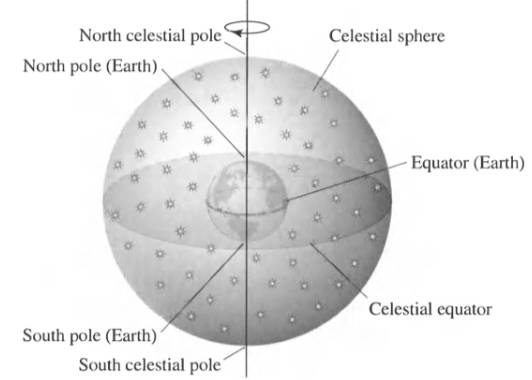
\includegraphics[width=6cm]{chapters/01/celestialsphere}
	\caption{天球,地球在中央,天球赤道和地球赤道共面。}
	\label{fig:celestialsphere}
\end{figure}


\begin{figure}[hbt]
  \centering
  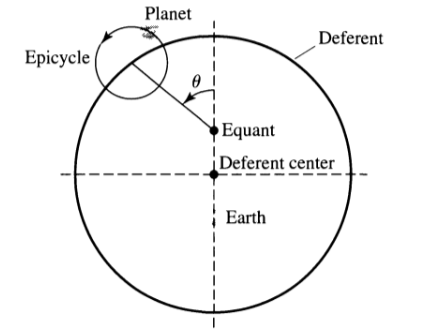
\includegraphics[width=6cm]{chapters/01/ptolemaicmodel}
  \caption{提出本轮、均轮、equant来解释{\bf 逆行运动}	}
  \label{fig:ptolemarcmodel}
\end{figure}

\section{日心说}
内行星:位于地球轨道以内的行星。相对于太阳最大的角间距称为{\bf 东、西大距},此时视亮度最大。

外行星:位于地球轨道以外的行星。亮度最大处称为照。

合:从地球上看,跑到太阳一侧,对于内行星,在太阳背后叫上合,在太阳前面叫下合

冲:从地球上看,跑到太阳反方向

会合周期(S):相邻两次冲或合(相对地球)的时间间隔

恒星周期(P):完成一次公转所需要的时间

\begin{displaymath}
  1/S=
  \begin{dcases}
  	1/P-1/P_{\oplus}\ \text{(内行星)} \\
  	1/P_{\oplus}-1/P\ \text{(外行星)}
  \end{dcases}
\end{displaymath}

\section{天球坐标}\label{sec:celestial}
\subsection{高度方位坐标系}
\begin{figure}[hbt]
  \centering
  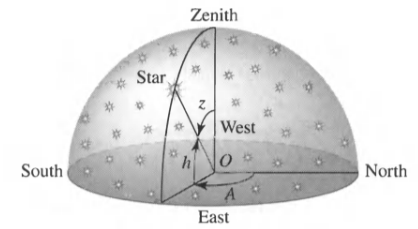
\includegraphics[width=6cm]{chapters/01/altitude}
  \caption{高度方位坐标系}
  \label{fig:altitude}
\end{figure}

高度角$h$:天体与水平面的夹角,如图\ref{fig:altitude}

天顶:观测者正上方

天顶距$z$:天体与天顶的夹角

方位角$A$:从某点的指北方向线(通常用子午线,即经线)起依顺时针(东)方向至目标方向线间的水平夹角

地球的自转轨道面(赤道面)和公转轨道面(黄道面)存在夹角(黄赤交角),因此在一年中太阳的直射点会发生变化,由此定义春分点、夏至点、秋分点、冬至点。

太阳时:太阳经过子午线的平均间隔(考虑地球自转)

恒星时:背景恒星经过子午线的平均间隔

\subsection{赤道坐标系}

\begin{figure}[hbt]
  \centering
  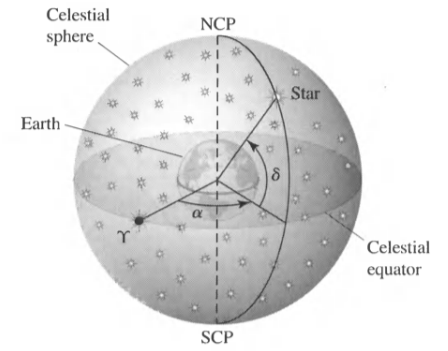
\includegraphics[width=6cm]{chapters/01/equatorial}
  \caption{赤道坐标系}
  \label{fig:equatorial}
\end{figure}
赤纬$\delta$:等价于纬度

赤经$\alpha$:自春分点依顺时针(东)方向至被测点所在时圈的时差,一周24小时等价于360$^\circ$,1h=15$^\circ$,1m=15$'$
,1s=15$''$

本地恒星时:观测者所在子午线的赤经

{\bf
进动(岁差)}会导致天体的赤经、赤纬发生变化(因为春分点发生变化),因此要确定一个特定的时期来确定春分点的变化,对赤道坐标作出修正
,这个时期被定义为2000年1月1日正午英国格林尼治的观测值(J2000.0)

\begin{align}
  \Delta\alpha &=M+N \sin\alpha \tan\delta \\
  \Delta\delta &=N\cos\alpha
\end{align}

其中

\begin{align}
  M &=1^\circ.2812323T+0.^\circ0003879T^2+0.^\circ0000101T^3 \notag \\
  N &=0^\circ.5567530T-0.^\circ0001185T^2-0.^\circ0000116T^3 \notag
\end{align}

其中$T$定义为

\begin{equation}
  T=(t-2000.0)/100
\end{equation}

其中$t$是当前时间,以年的分数来表示。

\subsection{自行}
天体本身通常具有相对太阳运动,其速度可分解为视向速度$v_r$和切向速度$v_\theta$,而切向速度会导致天体的坐标发生变化,这种运动被称为{\bf 自行}
\begin{displaymath}
  \mu\equiv{d\theta\over dt} ={v_\theta \over r}
\end{displaymath}

\begin{figure}[hbt]
  \centering
  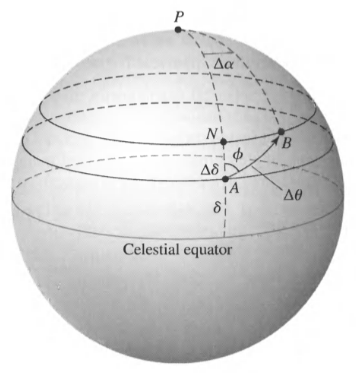
\includegraphics[width=6cm]{chapters/01/propermotion}
  \caption{自行示意图}
  \label{fig:proper}
\end{figure}


考虑到在天球上运动的几何关系如图\ref{fig:proper},且天体是沿位置角$\phi$运动,可以得到
\begin{align}
   \Delta\alpha &=\Delta\theta{\sin \phi \over \cos \delta}\\
   \Delta\delta &=\Delta\theta\cos\phi\\
   (\Delta\theta)^2 &=(\Delta\alpha\cos\delta)^2+(\Delta\delta)^2
\end{align}
